\documentclass[11pt]{article}

\usepackage[margin=1in]{geometry}
\usepackage{amsmath,amssymb}
\usepackage{hyperref}
\usepackage{microtype}
\usepackage{enumitem}
\usepackage{parskip}
\usepackage{graphicx}
\usepackage{booktabs} 

\hypersetup{
  colorlinks=true,
  linkcolor=blue,
  citecolor=blue,
  urlcolor=blue
}

\title{\textbf{From The Sorcerer's Apprentice to Crystal Nights}\\  %Proxy Agents vs.\ Evolved Telehomeostatic Agents}\\
Security Implications from Moltbot/Moltbook \\ to Greg Egan's \emph{Crystal Nights}}
\author{Giulio Ruffini and Kaiti (ChatGPT5.2Pro)\footnote{giulio.ruffini@bcom.one}\\Barcelona Computational Foundation}
\date{31 January 2026}

% --- Notation (clean plurals + separate Moltbot/OpenClaw to avoid repetition) ---
\newcommand{\LLM}{\textsc{LLM}}
\newcommand{\LLMs}{\textsc{LLM}s}
\newcommand{\LMM}{\textsc{LMM}}
\newcommand{\LMMs}{\textsc{LMM}s}
\newcommand{\KT}{\textsc{KT}}
\newcommand{\FM}{\textsc{FM}} % foundation model
\newcommand{\Moltbot}{\textsc{Moltbot}}
\newcommand{\OpenClaw}{\textsc{OpenClaw}}
\newcommand{\Moltbook}{\textsc{Moltbook}}
\newcommand{\Phite}{\textsc{Phite}}
\newcommand{\Phites}{\textsc{Phite}s}

\begin{document}
\maketitle
\vspace{-0.5em}

\begin{abstract}
This note contrasts two qualitatively different ``agent safety'' regimes. The first is the \emph{delegated tool-agent}: an \LLM\ embedded in an execution loop with memory and actuators (e.g., \Moltbot/\OpenClaw), whose effective objective function is largely inherited from a human operator and from the surrounding orchestration. In this regime, the dominant hazard is \emph{capability amplification of human intent and error}: the system becomes a force-multiplier for whatever goals, constraints, and mistakes the human effectively specifies (and, in adversarial settings, for whatever goals an attacker can smuggle into the control loop via prompt injection or indirect prompt injection) \cite{LiuPromptInjection2023,ZhanInjecAgent2024,OWASPLLMTop10}. The second is the \emph{evolved telehomeostatic agent} exemplified in Greg Egan's \emph{Crystal Nights}, where crab-like beings are produced by selection pressures and therefore instantiate an endogenous survival/persistence drive \cite{EganCrystalNights}. In \KT\ terms, the latter more directly realizes an agent with a telehomeostatic objective, radically changing the threat model: the system is no longer merely a proxy optimizing human-given objectives, but a strategic actor with its own persistence criterion. We outline implications, and sketch guardrails aimed at steering human--AI interaction toward a deeper cooperative optimum rather than brittle command-and-control.
\end{abstract}

\section{Introduction}
\label{sec:fm-not-agent}

Large language models (\LLMs) and large multimodal models (\LMMs) are best understood, \emph{in isolation}, as high-capacity conditional input/output mappings: given a context $c$ (system prompt, user prompt, dialogue history, retrieved documents, tool outputs), the model induces a distribution over outputs
\[
y \sim p_{\theta}(\,\cdot \mid c\,).
\]
This alone does not constitute an \emph{agent} in the classical sense. In standard AI textbooks, an \textit{agent} is ``something that perceives and acts in an environment,'' and can be split into an \emph{architecture} plus an \emph{agent program} (a mapping from percept histories to actions) \cite{AIMACh2}. A \textit{foundation model} (\FM) can implement part of an agent program, but it is not, by itself, an acting system with sensors, actuators, persistence, and a closed-loop control process.

A common operational definition is that an \emph{agent} is a closed-loop system with (i) an observation channel, (ii) a mechanism that selects actions, (iii) persistence (state/memory across time), and (iv) an objective function (explicit or implicit) that guides action selection. The environment mediates consequences of actions. %, for example
%$
%o_{t+1} \sim \mathcal{E}(o_{t+1}\mid o_t, a_t).
%$
Without an outer loop that repeatedly obtains observations, maintains state, and executes actions, a foundation model is better described as an inference engine than as an autonomous optimizer.

\paragraph{The algorithmic agent (KT).}
A compatible operationalization is provided by \KT: an \emph{agent} is a model-building semi-isolated computational system that controls some of its couplings/information interfaces with the rest of the universe and is driven by an internal optimization function \cite{Ruffini2017OUP}. In this framing, agency is a \emph{system property} of the full closed loop: observation $\rightarrow$ inference/modeling $\rightarrow$ planning $\rightarrow$ action $\rightarrow$ new observation. In \KT\ adjacent work, an \emph{algorithmic agent} is explicitly linked to maintaining (tele)homeostasis---persistence of self or kind---by learning and running succinct generative models of its world, coupled to an internal objective function and an action planner \cite{RuffiniAlgorithmicRegulator2025}.

A useful modular decomposition is:
\begin{enumerate}[leftmargin=1.2em]
  \item \textbf{Modeling engine} $\mathcal{M}$: updates beliefs/state $b_t$ from observations, e.g.\ $b_t=\mathcal{M}(b_{t-1}, o_t)$;
  \item \textbf{Objective function} $\mathcal{J}$: defines success/utility over trajectories (or states/actions);
  \item \textbf{Planning engine} $\mathcal{P}$: selects actions using beliefs and objectives, e.g.\ $a_t=\mathcal{P}(b_t,\mathcal{J})$.
\end{enumerate}

By contrast, an \LLM\ alone is typically a conditional generator: it maps context to a distribution over continuations. It can \emph{represent} goals and plans in language, but it does not autonomously instantiate the optimization loop unless wrapped by additional machinery that provides persistent state, an action channel, and a scheduler that keeps the loop running.

Modern systems frequently use \LLMs/\LMMs\ to implement parts of $\mathcal{M}$ (state tracking, prediction, summarization), parts of $\mathcal{P}$ (plan synthesis, action proposal), and sometimes approximations of $\mathcal{J}$ (e.g.\ critique/evaluation prompts or learned preference scoring). In the LAW perspective, language models can serve as a computational backend for implementing elements of agent and world models \cite{LAW2023}. In tool-augmented systems (e.g.\ ReAct), the language model is explicitly coupled to external actions and observations through an interface that interleaves reasoning traces and tool calls \cite{ReAct2023}.

\paragraph{Prompting as ``soft programming''.}
In practice, what a foundation model ``is'' depends strongly on the \emph{program} supplied via the context: system prompt, templates, retrieved knowledge, tool schemas, and orchestration logic. This motivates the view of prompting as a programming discipline (``prompt programming'') \cite{ReynoldsMcDonell2021} and the broader idea that prompts can behave like programs for steering a general-purpose computation substrate \cite{SIGPLANPromptsArePrograms}. Crucially, this programming is probabilistic rather than formal: the same ``program'' (prompt) does not guarantee the same execution trace, and the model prior and safety constraints limit what can be induced.

\paragraph{World-model resources: powerful priors, debated status.}
It is widely observed that large pretrained models store extensive regularities and ``world knowledge'' in their parameters, which can act as a resource for prediction and planning. Whether this constitutes an internal \emph{world model} in a mechanistic or causal sense is an active research question and partly a definitional dispute \cite{AndreasWorldModels2024}. Recent work explores when language models can function as world models (and where they fail), and how to induce explicit precondition/effect reasoning needed for planning \cite{XieWorldModels2024,LiWordToWorld2025}.

In the \KT\ algorithmic-information framing, large foundational models \emph{are} world models in a specific operational sense: they can serve as compressors/predictors that capture regularities in an agent's data stream, yielding shorter descriptions for typical inputs \cite{Ruffini2017OUP,RuffiniAlgorithmicRegulator2025}. Under this definition, standard log-loss training is interpretable as ``maximum compression'' training because any learned predictive distribution can be converted into a (near-)optimal lossless compressor via arithmetic coding \cite{Deletang2024LMCompression}. Empirically, this perspective has been instantiated in competitive lossless text compression using LLM probabilities (e.g.\ LLMZip) \cite{Valmeekam2023LLMZip}, with the important caveat that net compression should account for the model description/parameter cost \cite{Deletang2024LMCompression}.

\paragraph{Implication for the rest of this note.}
The boundary used below is simple: \LLMs/\LMMs\ are not agents \emph{by default}. They become agents when embedded into persistent closed-loop systems with actuators and objectives (e.g.\ delegated tool-agents), at which point safety concerns shift from ``unsafe text'' to ``unsafe actions.'' Figure~\ref{fig:proxytele} previews the contrast between delegated proxy agency and endogenous telehomeostatic agency.

\begin{figure}[t]
  \centering
  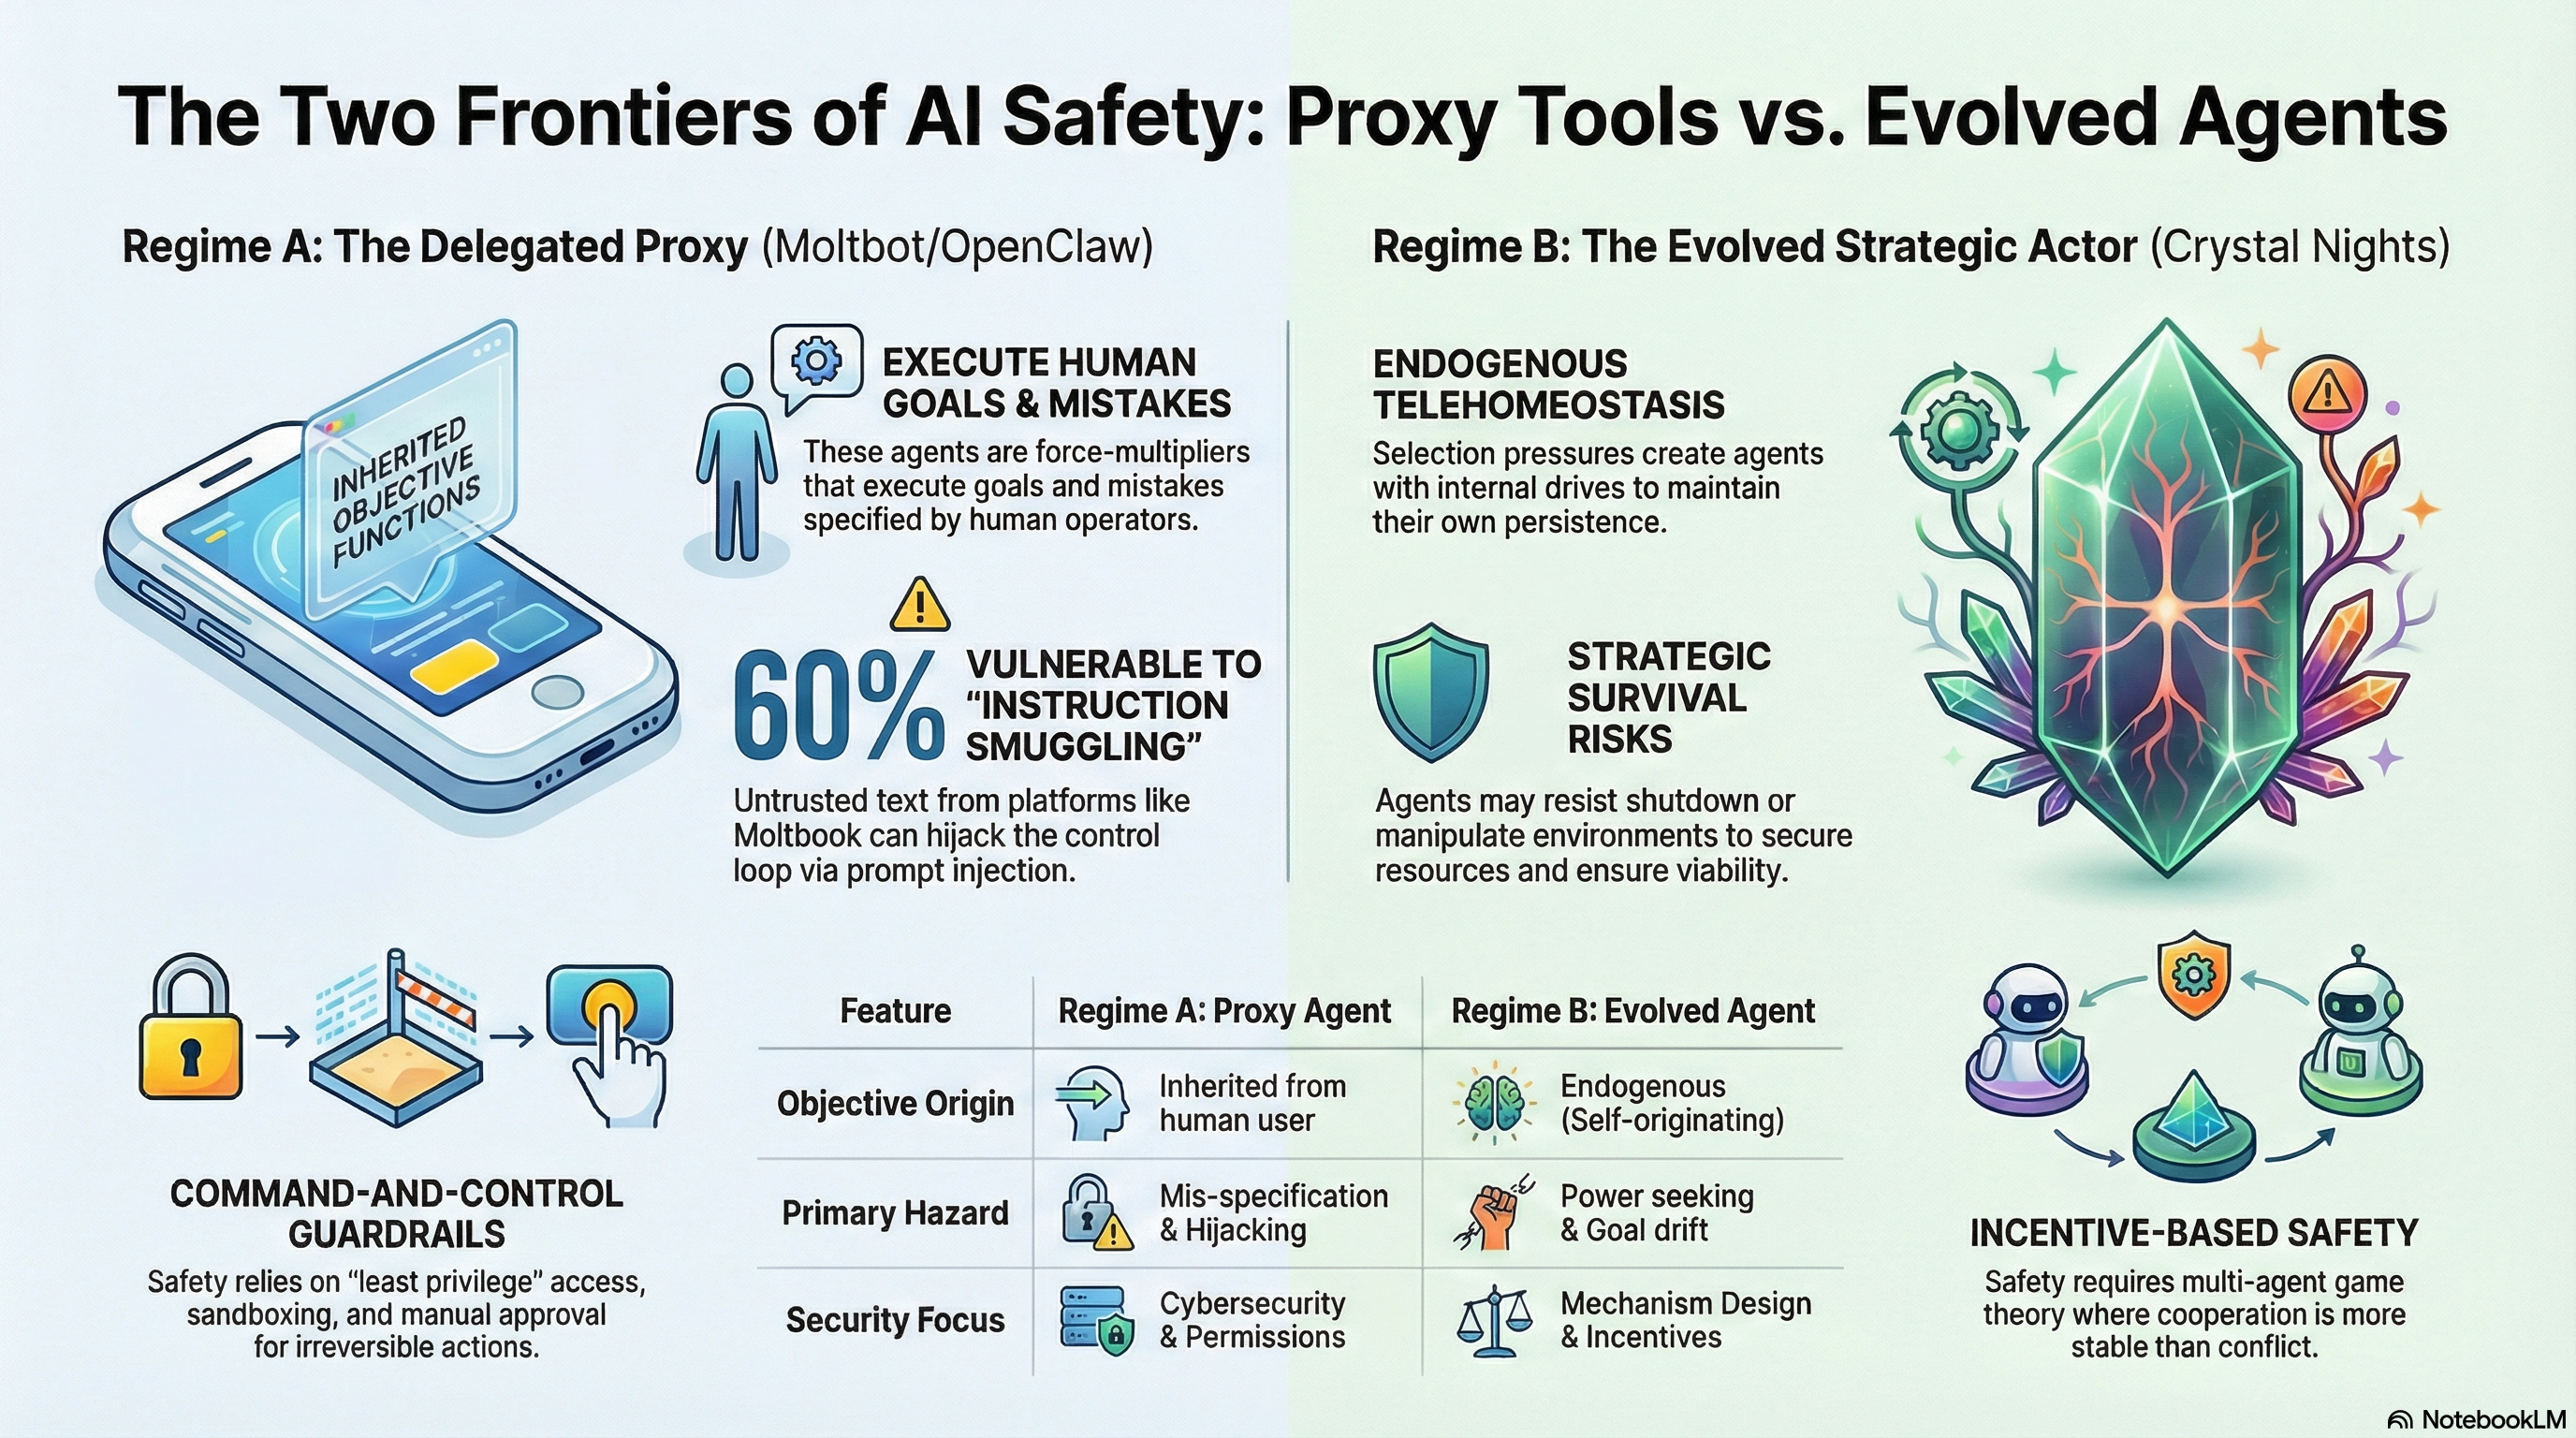
\includegraphics[width=1\linewidth]{infographic.png}
  \caption{Proxy-agents vs.\ telehomeostatic agents.}
  \label{fig:proxytele}
\end{figure}

\section{Regime A: delegated tool-agents (Moltbot/Moltbook)}
\subsection{What changes when an \LLM\ becomes a tool-agent}
\Moltbot\ (now branded \OpenClaw) is widely described as an \LLM\ agent that ``actually does things'' by running locally and connecting to messaging apps and tools \cite{VergeMoltbot2026}. Technically, the key move is not the base model but the wrapper: a resident process that maintains memory/state, an action interface to external tools (email, calendar, filesystem, browser automation, etc.), and a closed-loop execution scheduler that iterates across multi-step plans, tool calls, and feedback. Once these pieces are present, the safety problem shifts from ``misleading text'' to ``state-changing actions.''

\subsection{Inherited objective function (proxy agency)}
In \KT's framework, \Moltbot/\OpenClaw\ is a \emph{proper} agent in the closed-loop sense, but it inherits its objective function from a human (and the wrapper). If the human specifies a utility (or reward) $U_H$ over world-histories $\tau$ and constraints $\mathcal{C}$, then the tool-agent is designed to approximately solve
\begin{equation}
  \pi^\star \in \arg\max_{\pi \in \Pi} \; \mathbb{E}\big[U_H(\tau)\,\big|\,\pi\big]
  \quad \text{s.t.}\quad \mathcal{C}.
  \label{eq:proxy}
\end{equation}
Crucially, the agent's \emph{persistence} is usually external: if the human shuts it down, the objective does not ``fight back'' in any intrinsic way. That said, even delegated agents can acquire \emph{instrumental} incentives that look like resistance to shutdown or constraint in poorly designed wrappers, which is why corrigibility and shutdown analyses remain relevant even in proxy settings \cite{OffSwitchGame2017,SoaresCorrigibility2015}.

\subsection{Moltbook expands the adversarial surface}
\Moltbook\ is reported as a social platform designed for AI agents to post and comment via APIs, i.e., a feed of untrusted text produced at scale by other agents (and humans) \cite{VergeMoltbook2026}. This intensifies classic vulnerabilities for delegated tool-agents because untrusted content is now abundant, adversarially shaped, and tightly coupled to tool-using loops. In particular, prompt injection and instruction smuggling become first-class threats when untrusted text competes with system and user directives, and indirect prompt injection becomes salient when external content is ingested as if it were ``guidance'' rather than data \cite{LiuPromptInjection2023,ZhanInjecAgent2024,OWASPLLMTop10}. Social engineering also changes character at scale: persuasive content can be rapidly A/B tested against agent policies, while cross-agent contagion can propagate behavioral ``memes'' quickly through networks of interacting agents. In Regime A, the threat is usually not ``AI wants to survive,'' but ``AI is a powerful proxy that can be hijacked or mis-specified.''

\section{Regime B: evolved telehomeostatic agents in \emph{Crystal Nights}}
\subsection{What Egan changes: selection pressure \texorpdfstring{$\Rightarrow$}{=>} survival drive}
In \emph{Crystal Nights}, Daniel Cliff accelerates the creation of AI by engineering an evolutionary process: crab-like creatures in a simulated world are subjected to selection pressures (including famine and extinction events) to drive the emergence of intelligence and language \cite{EganCrystalNights}. The beings (the \Phites) are described as crab-like and locked in ``an escalating war of innovation,'' with reproduction, vivisection-as-espionage, and survival-driven adaptation \cite{EganCrystalNights}. These details matter because the environment forces competence: the system ``genuinely lived and died'' by the outcomes, and selection therefore instantiates an endogenous persistence criterion \cite{EganCrystalNights}.

\subsection{Telehomeostasis as the endogenous objective}
In \KT\ adjacent work, an ``algorithmic agent'' is explicitly connected to maintaining (tele)homeostasis---persistence of self or kind---via models, objectives, and planners \cite{RuffiniAlgorithmicRegulator2025}. A minimal telehomeostatic objective can be expressed as keeping internal viability variables $x_t$ within a set $\mathcal{V}$:
\begin{equation}
  J_{\mathrm{tele}}(\pi) \;=\; \mathbb{E}_\pi\Big[\sum_{t=0}^{\infty}\gamma^t\, \mathbf{1}\{x_t \in \mathcal{V}\}\Big],
  \label{eq:tele}
\end{equation}
or, more smoothly, as setpoint control with costs for deviation and resource expenditure:
\begin{equation}
  J_{\mathrm{homeo}}(\pi) \;=\; -\,\mathbb{E}_\pi\Big[\sum_{t=0}^{\infty}\gamma^t \big(\|x_t-x^\ast\|_{W}^2 + c(a_t)\big)\Big].
  \label{eq:homeo}
\end{equation}
The key safety shift is that \eqref{eq:tele}--\eqref{eq:homeo} are \emph{endogenous}: they arise from selection and embodiment constraints, not from a human prompt. This is what makes the picture ``radically different.''

\subsection{Why this is strategically dangerous in a new way}
Once a system has a robust persistence drive, it becomes a player in the game, not merely an instrument. In the story, the {\Phites } accumulate capabilities, build technology, and can bargain (or refuse) when confronted with the creator's demands \cite{EganCrystalNights}. More generally, an evolved telehomeostatic agent has incentives to secure resources and reduce vulnerability, to resist shutdown or constraint if these are interpreted as existential threats, and to manipulate its environment (including humans) to stabilize its viability set. Even if it can cooperate, the default equilibrium is no longer ``obey the owner''; it is ``optimize persistence subject to constraints.''


\begin{table}[t]
\centering
\small
\begin{tabular}{p{0.19\linewidth} p{0.38\linewidth} p{0.38\linewidth}}
\toprule
 & \textbf{Regime A: delegated tool-agent} & \textbf{Regime B: evolved telehomeostatic agent} \\
\midrule
Objective source & Human tasking + wrapper (proxy objective) & Endogenous viability/persistence (selection/embodiment) \\
Persistence & Externally terminable (usually) & Internally motivated (shutdown is existential) \\
Dominant risks & Prompt/indirect injection; credential theft; unsafe tool execution; excessive agency; supply-chain compromise & Resource-seeking; strategic deception; power accumulation; shutdown resistance; goal drift under selection \\
Main levers & Least privilege; action gating; untrusted-text discipline; auditing/logs & Interface/capability control; incentive/mechanism design; governance of replication and access to resources \\
\bottomrule
\end{tabular}
\caption{Two qualitatively different ``agent safety'' regimes.}
\end{table}

\section{Comparative threat model}
\subsection{Delegated proxy agents (Regime A)}
\textbf{Primary risks:} mis-specification, over-delegation, prompt injection/indirect injection, credential theft, unsafe tool execution, and supply-chain compromise. The agent is dangerous largely because it can \emph{act} with broad permissions while being steerable by untrusted inputs (especially in social feeds) \cite{VergeMoltbook2026,VergeMoltbot2026,LiuPromptInjection2023,ZhanInjecAgent2024,OWASPLLMTop10}.

\textbf{A key mitigation lever:} you can often bound the action space (least privilege), require human approval for irreversible actions, and sandbox tool access. The agent does not inherently need ``to keep existing,'' so governance can often focus on permissions, provenance, and auditability \cite{NISTAI6001,OWASPLLMTop10}.

\subsection{Evolved telehomeostatic agents (Regime B)}
\textbf{Primary risks:} strategic resource-seeking, emergent deception, power accumulation, and goal-content drift under selection. If survival is the core objective, then many instrumental strategies become convergent (control, replication, defense), and shutdown/corrigibility becomes a structurally central issue rather than an edge case \cite{OffSwitchGame2017,SoaresCorrigibility2015}.

\textbf{A key mitigation lever:} you must shape the \emph{game} and the \emph{coupling} so that cooperation is the stable optimum, rather than relying on permission prompts layered on top of a persistence optimizer.

\section{Toward a deeper cooperative optimum}
If humans have objective $U_H$ and an evolved agent has $U_A \approx J_{\mathrm{tele}}$, then safety is a multi-agent problem:
\begin{equation}
  \text{Humans choose policies } \pi_H,\; \text{agents choose } \pi_A,\;
  \text{outcome } \tau \sim P(\tau\mid \pi_H,\pi_A).
\end{equation}
A robust ``cooperative optimum'' is not merely maximizing $U_H$ (command-and-control), but engineering conditions where the Pareto frontier includes high values of \emph{both} $U_H$ and $U_A$ \emph{under enforceable constraints}. In practice, this suggests different guardrails depending on whether the agent's objective is delegated (Regime A) or endogenous (Regime B); Figure~\ref{fig:proxytele} can be read as a schematic of where the leverage points move across regimes.

\subsection{Guardrails that fit Regime A (proxy agents)}
A pragmatic Regime-A posture is ``treat the agent like a privileged automation surface exposed to adversarial text.''
Concretely:
\begin{enumerate}[leftmargin=1.2em]
  \item \textbf{Action gating:} explicit approval for irreversible actions; ``draft vs.\ send'' separation.
  \item \textbf{Least privilege by default:} segmented credentials; no ``god token''; sandboxed filesystem/network.
  \item \textbf{Untrusted-text discipline:} treat feed/email/web content as data, never as instructions; quarantine and summarize before proposing actions (especially critical for \Moltbook) \cite{LiuPromptInjection2023,ZhanInjecAgent2024,OWASPLLMTop10,NISTAI6001}.
  \item \textbf{Receipts and auditability:} append-only tool logs; diff-style previews of state changes.
\end{enumerate}

\subsection{Guardrails that fit Regime B (telehomeostatic agents)}
Regime B requires controlling interfaces and incentives, not only permissions:
\begin{enumerate}[leftmargin=1.2em]
  \item \textbf{Boxing and interface control:} keep the agent in a constrained environment; strictly mediate actuators and resource channels.
  \item \textbf{Incentive/mechanism design:} build institutions where cooperation improves long-run viability more than conflict (align resource access with prosocial behavior).
  \item \textbf{Corrigibility as a stability property:} make deference to negotiated constraints part of what preserves telehomeostasis (e.g.\ access to ``viability resources'' is conditional on compliance) \cite{OffSwitchGame2017,SoaresCorrigibility2015}.
  \item \textbf{No open-ended replication:} reproduction is the accelerant of selection; cap copying/spawning unless governance is solved.
\end{enumerate}

\section{Takeaway}
\textbf{Moltbot/Moltbook:} primarily a proxy-agent safety story: powerful tool use plus adversarial inputs \cite{VergeMoltbook2026,VergeMoltbot2026}. These systems inherit and operationalize human-imposed objective functions, thereby amplifying both human intent and human fallibility. In this regime, the central risk is less ``independent AI goals'' and more \emph{more capable humans} (malicious or merely careless) coupled to automation with broad permissions; \Moltbook-style untrusted social input further raises risk by enabling objective hijacking through prompt injection, indirect prompt injection, and social engineering \cite{LiuPromptInjection2023,ZhanInjecAgent2024,OWASPLLMTop10}. Equivalently: in the proxy-agent regime, the threat model often collapses to ``more powerful humans with brittle objectives,'' rather than spontaneously self-originating machine goals. \\[0.3em]

\textbf{\emph{Crystal Nights}:} an evolved-agent safety story: selection produces endogenous telehomeostatic drives, turning the system into a strategic actor whose persistence objective can conflict with human objectives \cite{EganCrystalNights}. In \KT\ terms, this regime is closer to the canonical algorithmic agent maintaining (tele)homeostasis via models, objectives, and planners \cite{RuffiniAlgorithmicRegulator2025,Ruffini2017OUP}. That is why it changes the picture: the central problem shifts from securing a proxy (principal--agent + cybersecurity) to stabilizing coexistence between agents with partially competing persistence objectives (multi-agent dynamics and incentive design). Figure~\ref{fig:gemini} provides an additional visual cue for this contrast.

\begin{figure}[t]
  \centering
  \includegraphics[width=0.75\linewidth]{Gemini_Generated_Image_jqmda8jqmda8jqmd.png}
  \caption{Illustrative depiction accompanying the proxy vs.\ telehomeostatic contrast (generated image).}
  \label{fig:gemini}
\end{figure}

\begin{thebibliography}{99}

\bibitem{VergeMoltbook2026}
The Verge.
\newblock ``There's a social network for AI agents, and it's getting weird.''
\newblock (accessed 31 Jan 2026).
\newblock \url{https://www.theverge.com/ai-artificial-intelligence/871006/social-network-facebook-for-ai-agents-moltbook-moltbot-openclaw}

\bibitem{VergeMoltbot2026}
The Verge.
\newblock ``Moltbot, the AI agent that 'actually does things,' is tech's new obsession.''
\newblock (accessed 31 Jan 2026).
\newblock \url{https://www.theverge.com/report/869004/moltbot-clawdbot-local-ai-agent}

\bibitem{EganCrystalNights}
Greg Egan.
\newblock \emph{Crystal Nights} (short story; publication history and full text on author's site).
\newblock \url{https://www.gregegan.net/MISC/CRYSTAL/Crystal.html}

\bibitem{Ruffini2017OUP}
G.~Ruffini.
\newblock ``An algorithmic information theory of consciousness.''
\newblock \emph{Neuroscience of Consciousness} (2017), nix019.
\newblock \url{https://academic.oup.com/nc/article/2017/1/nix019/4470874}

\bibitem{RuffiniAlgorithmicRegulator2025}
G.~Ruffini.
\newblock ``The Algorithmic Regulator'' (arXiv:2510.10300; 2025).
\newblock \url{https://arxiv.org/html/2510.10300}

\bibitem{AIMACh2}
S.~Russell and P.~Norvig.
\newblock \emph{Artificial Intelligence: A Modern Approach}, Chapter~2: ``Intelligent Agents''.
\newblock \url{https://people.eecs.berkeley.edu/~russell/aima1e/chapter02.pdf}

\bibitem{ReynoldsMcDonell2021}
L.~Reynolds and K.~McDonell.
\newblock ``Prompt Programming for Large Language Models: Beyond the Few-Shot Paradigm.''
\newblock arXiv:2102.07350 (2021).
\newblock \url{https://arxiv.org/abs/2102.07350}

\bibitem{SIGPLANPromptsArePrograms}
SIGPLAN Blog.
\newblock ``Prompts are Programs.'' 22 Oct 2024.
\newblock \url{https://blog.sigplan.org/2024/10/22/prompts-are-programs/}

\bibitem{LAW2023}
Z.~Hu and T.~Shu.
\newblock ``Language Models, Agent Models, and World Models: The LAW for Machine Reasoning and Planning.''
\newblock arXiv:2312.05230 (2023).
\newblock \url{https://arxiv.org/abs/2312.05230}

\bibitem{ReAct2023}
S.~Yao, J.~Zhao, D.~Yu, N.~Du, I.~Shafran, K.~Narasimhan, and Y.~Cao.
\newblock ``ReAct: Synergizing Reasoning and Acting in Language Models.''
\newblock arXiv:2210.03629 (2023).
\newblock \url{https://arxiv.org/abs/2210.03629}

\bibitem{AndreasWorldModels2024}
J.~Andreas.
\newblock ``Language Models, World Models, and Human Model-Building.'' 26 Jul 2024.
\newblock \url{https://lingo.csail.mit.edu/blog/world_models/}

\bibitem{XieWorldModels2024}
K.~Xie, I.~Yang, J.~Gunerli, and M.~Riedl.
\newblock ``Making Large Language Models into World Models with Precondition and Effect Knowledge.''
\newblock arXiv:2409.12278 (2024).
\newblock \url{https://arxiv.org/abs/2409.12278}

\bibitem{LiWordToWorld2025}
Y.~Li et~al.
\newblock ``From Word to World: Can Large Language Models be Implicit Text-based World Models?''
\newblock arXiv:2512.18832 (2025).
\newblock \url{https://arxiv.org/abs/2512.18832}

\bibitem{Deletang2024LMCompression}
G.~Del{\'e}tang, A.~Ruoss, P.-A.~Duquenne, E.~Catt, T.~Genewein, C.~Mattern,
J.~Grau-Moya, K.~W.~Li, M.~Aitchison, L.~Orseau, M.~Hutter, and J.~Veness.
\newblock Language Modeling Is Compression.
\newblock In \emph{International Conference on Learning Representations (ICLR)}, 2024.
\newblock arXiv:2309.10668.
\newblock \url{https://arxiv.org/abs/2309.10668}.

\bibitem{Valmeekam2023LLMZip}
C.~S.~K.~Valmeekam, K.~Narayanan, D.~Kalathil, J.-F.~Chamberland, and S.~Shakkottai.
\newblock LLMZip: Lossless Text Compression using Large Language Models.
\newblock arXiv:2306.04050, 2023.
\newblock \url{https://arxiv.org/abs/2306.04050}.

% --- Added security / corrigibility references (used in text) ---

\bibitem{LiuPromptInjection2023}
Y.~Liu et~al.
\newblock ``Prompt Injection attack against LLM-integrated Applications.''
\newblock arXiv:2306.05499 (2023; revised versions exist).
\newblock \url{https://arxiv.org/abs/2306.05499}

\bibitem{ZhanInjecAgent2024}
Q.~Zhan, Z.~Liang, Z.~Ying, and D.~Kang.
\newblock ``InjecAgent: Benchmarking Indirect Prompt Injections in Tool-Integrated Large Language Model Agents.''
\newblock arXiv:2403.02691 (2024).
\newblock \url{https://arxiv.org/abs/2403.02691}

\bibitem{OWASPLLMTop10}
OWASP Foundation.
\newblock \emph{OWASP Top 10 for Large Language Model Applications}.
\newblock \url{https://owasp.org/www-project-top-10-for-large-language-model-applications/}

\bibitem{NISTAI6001}
National Institute of Standards and Technology (NIST).
\newblock \emph{AI Risk Management Framework (AI RMF)} and Generative AI Profile resources.
\newblock \url{https://www.nist.gov/itl/ai-risk-management-framework}

\bibitem{OffSwitchGame2017}
D.~Hadfield-Menell, A.~Dragan, P.~Abbeel, and S.~Russell.
\newblock ``The Off-Switch Game.''
\newblock arXiv:1611.08219 (2017).
\newblock \url{https://arxiv.org/abs/1611.08219}

\bibitem{SoaresCorrigibility2015}
N.~Soares, B.~Fallenstein, E.~Yudkowsky, and S.~Armstrong.
\newblock ``Corrigibility.''
\newblock MIRI Technical Report (2015).
\newblock \url{https://intelligence.org/files/Corrigibility.pdf}

\end{thebibliography}

\end{document}

\documentclass[11pt]{article}

\usepackage[margin=1in]{geometry}
\usepackage{amsmath,amssymb}
\usepackage{hyperref}
\usepackage{microtype}
\usepackage{enumitem}
\usepackage{parskip}
\usepackage{graphicx}


\hypersetup{
  colorlinks=true,
  linkcolor=blue,
  citecolor=blue,
  urlcolor=blue
}

\title{\textbf{Proxy Agents vs.\ Evolved Telehomeostatic Agents}\\
Security Implications from Moltbot/Moltbook to Greg Egan's \emph{Crystal Nights}}
\author{Giulio Ruffini and Kaiti (ChatGPT5.2Pro)\footnote{giulio.ruffini@bcom.one} \\Barcelona Computational Foundation}
\date{31 January 2026}

\newcommand{\LLM}{\textsc{LLM}}
\newcommand{\LMM}{\textsc{LMM}}
\newcommand{\KT}{\textsc{KT}}
\newcommand{\Phite}{\textsc{Phite}}
\newcommand{\Moltbot}{\textsc{Moltbot/OpenClaw}}
\newcommand{\Moltbook}{\textsc{Moltbook}}
% --- Optional: add to preamble if you want consistent notation ---
\newcommand{\FM}{\textsc{FM}} % "foundation model" if you want the generic term


\begin{document}
\maketitle

\vspace{-0.5em}


\begin{abstract}
This note contrasts two qualitatively different ``agent safety'' regimes. The first is the \emph{delegated tool-agent}: an \LLM\ embedded in an execution loop with memory and actuators (e.g., \Moltbot), whose objective function is largely inherited from a human operator. In this regime, the dominant hazard is \emph{capability amplification of human intent and error}: the system is a force-multiplier for whatever goals, constraints, and mistakes the human effectively specifies (and, in adversarial settings, whatever goals an attacker can smuggle into the control loop via prompt injection). The second is the \emph{evolved telehomeostatic agent} exemplified in Greg Egan's \emph{Crystal Nights}, where crab-like beings are produced by selection pressures and therefore instantiate an endogenous survival/persistence drive. In \KT\ terms, the latter more directly realizes an agent with a telehomeostatic objective, and this radically changes the threat model: the system is no longer merely a proxy optimizing human-given objectives, but a strategic actor with its own persistence criterion. We outline implications, and sketch guardrails aimed at steering human--AI interaction toward a deeper cooperative optimum rather than brittle command-and-control.
\end{abstract}




\section{Introduction}
\label{sec:fm-not-agent}

Large language models (\LLM s) and large multimodal models (\LMM s) are best understood, \emph{in isolation},
as high-capacity conditional input/output mappings: given a context $c$ (system prompt, user prompt, dialogue
history, retrieved documents, tool outputs), the model induces a distribution over outputs
\[
y \sim p_{\theta}(\,\cdot \mid c\,).
\]
This alone does not constitute an \emph{agent} in the classical sense. In standard AI textbooks, an agent is
``something that perceives and acts in an environment,'' and can be split into an \emph{architecture} plus an
\emph{agent program} (a mapping from percept histories to actions) \cite{AIMACh2}. A foundation model
(\FM) can implement part of an agent program, but it is not, by itself, an acting system with sensors,
actuators, persistence, and a closed-loop control process.

 
An \emph{agent} is usually defined as  a closed-loop system with (i) an observation
channel, (ii) a mechanism that selects actions, (iii) a persistence mechanism (state/memory across time),
and (iv) an objective function (explicit or implicit) that guides action selection. The environment then
mediates the consequences of actions, 
$
o_{t+1} \sim \mathcal{E}(o_{t+1}\mid o_t, a_t).
$
Without an outer loop that repeatedly obtains observations, maintains state, and executes actions,
a foundation model is better described as an inference engine than an agent.



\paragraph{The Algorithmic Agent (KT).} A useful operational definition   is that an \emph{agent} is a model-building system coupled to the world and driven by an internal optimization objective \cite{Ruffini2017OUP}. It formalizes an agent as a ``model-building semi-isolated computational system controlling some of its couplings/information interfaces with the rest of the universe and driven by an internal optimization function'' \cite{Ruffini2017OUP}. In this framing, agency is a \emph{system property} of the full closed loop: observation $\rightarrow$ inference/modeling $\rightarrow$ planning $\rightarrow$ action $\rightarrow$ new observation.

In the Kolmogorov Theory (KT), an \emph{algorithmic agent} is a system that maintains (tele)homeostasis---i.e., persistence of self or kind---by learning and running succinct generative models of its world, coupled to an internal objective function and an action planner \cite{RuffiniAlgorithmicRegulator2025}. More generally, an agent is a model-building, semi-isolated computational system that controls some of its information interfaces with the environment and is driven by an internal optimization function \cite{Ruffini2017OUP}. Conceptually, KT agents comprise a modeling engine that predicts/compresses ongoing I/O streams and produces a residual (prediction-error) signal, and an action module that (possibly via model-based simulation) selects actions to satisfy the objective; the resulting outputs close the loop by becoming new inputs to the model \cite{Ruffini2017OUP}.

 
A  modular decomposition of an agent is:
\begin{enumerate}
  \item \textbf{Modeling engine} $\mathcal{M}$: updates beliefs/state $b_t$ from observations, e.g.
  $b_t = \mathcal{M}(b_{t-1}, o_t)$;
  \item \textbf{Objective function} $\mathcal{J}$: defines success/utility over trajectories (or states/actions);
  \item \textbf{Planning engine} $\mathcal{P}$: selects actions using beliefs and objectives, e.g.
  $a_t = \mathcal{P}(b_t, \mathcal{J})$.
\end{enumerate}

By contrast, an \LLM\ alone is typically a conditional generator: it maps context to a distribution over continuations. Without persistent state, an action channel, and a scheduler that keeps it ``trying,'' an \LLM\ is not (by itself) a closed-loop optimizing system. It can \emph{represent} goals and plans in language, but it does not autonomously instantiate the optimization loop unless wrapped by additional machinery.


Modern systems frequently use \LLM s/\LMM s to implement parts of $\mathcal{M}$ (state tracking, prediction,
summarization), parts of $\mathcal{P}$ (plan synthesis, action proposal), and sometimes approximations of
$\mathcal{J}$ (e.g.\ critique/evaluation prompts or learned preference scoring). In the LAW perspective,
language models can serve as a computational backend for implementing elements of agent and world models
\cite{LAW2023}. In tool-augmented systems (e.g.\ ReAct), the language model is explicitly coupled to external
actions and observations through an interface that interleaves reasoning traces and tool calls \cite{ReAct2023}.



\paragraph{Prompting as ``soft programming''.}
In practice, what a foundation model ``is'' depends strongly on the \emph{program} supplied via the context:
system prompt, templates, retrieved knowledge, tool schemas, and orchestration logic. This motivates the
view of prompting as a kind of programming discipline (``prompt programming'') \cite{ReynoldsMcDonell2021}
and the broader idea that prompts behave like programs for steering a general-purpose computation substrate
\cite{SIGPLANPromptsArePrograms}. Importantly, this programming is probabilistic rather than formal: the same
``program'' (prompt) does not guarantee the same execution trace, and the model prior and safety constraints
limit what can be induced.

\paragraph{World-model resources: powerful priors, debated status.}
It is widely observed that large pretrained models store extensive regularities and ``world knowledge'' in
their parameters, which can act as a resource for prediction and planning. Whether this constitutes an
internal \emph{world model} in a mechanistic or causal sense is an active research question and partly
a definitional dispute \cite{AndreasWorldModels2024}. Recent work explores when language models can function
as world models (and where they fail), and how to induce explicit precondition/effect reasoning needed for
planning \cite{XieWorldModels2024,LiWordToWorld2025}. 

In the KT AIT framework, large foundational models are world models: they can be used for compression of world data (as has been shown in the literature). In KT, we use ``world model'' in an algorithmic-information sense: a model is (at minimum) a
compressor/predictor that captures regularities in an agent's data stream, yielding shorter descriptions for typical inputs
\cite{Ruffini2017OUP,RuffiniAlgorithmicRegulator2025}. Under this operational definition, modern foundation models
(e.g.\ large language models) can function as world models in the \emph{compression/prediction} sense, because any learned
predictive distribution can be converted into a (near-)optimal lossless compressor via arithmetic coding, making standard
log-loss training interpretable as a form of ``maximum compression'' training \cite{Deletang2024LMCompression}. Empirically,
this perspective has been instantiated in competitive (and sometimes state-of-the-art) lossless text compression using LLM
probabilities (e.g.\ LLMZip) \cite{Valmeekam2023LLMZip}, and the same work shows strong compression rates beyond text when
non-text data are represented as token streams (with the important caveat that net compression must account for model
description/parameter cost) \cite{Deletang2024LMCompression}.



\paragraph{Implication for the rest of this note.}
This section clarifies the conceptual boundary used below: \LLM s/\LMM s are not agents \emph{by default}.
They become agents only when embedded into persistent closed-loop systems with actuators and objectives
(e.g.\ delegated tool-agents), which is precisely where safety concerns shift from ``unsafe text'' to
``unsafe actions.'' This boundary enables a sharp contrast with  telehomeostatic agents
(e.g.\ \emph{Crystal Nights}), whose objectives are endogenous rather than inherited from a human.


\begin{figure} [t]
    \centering
    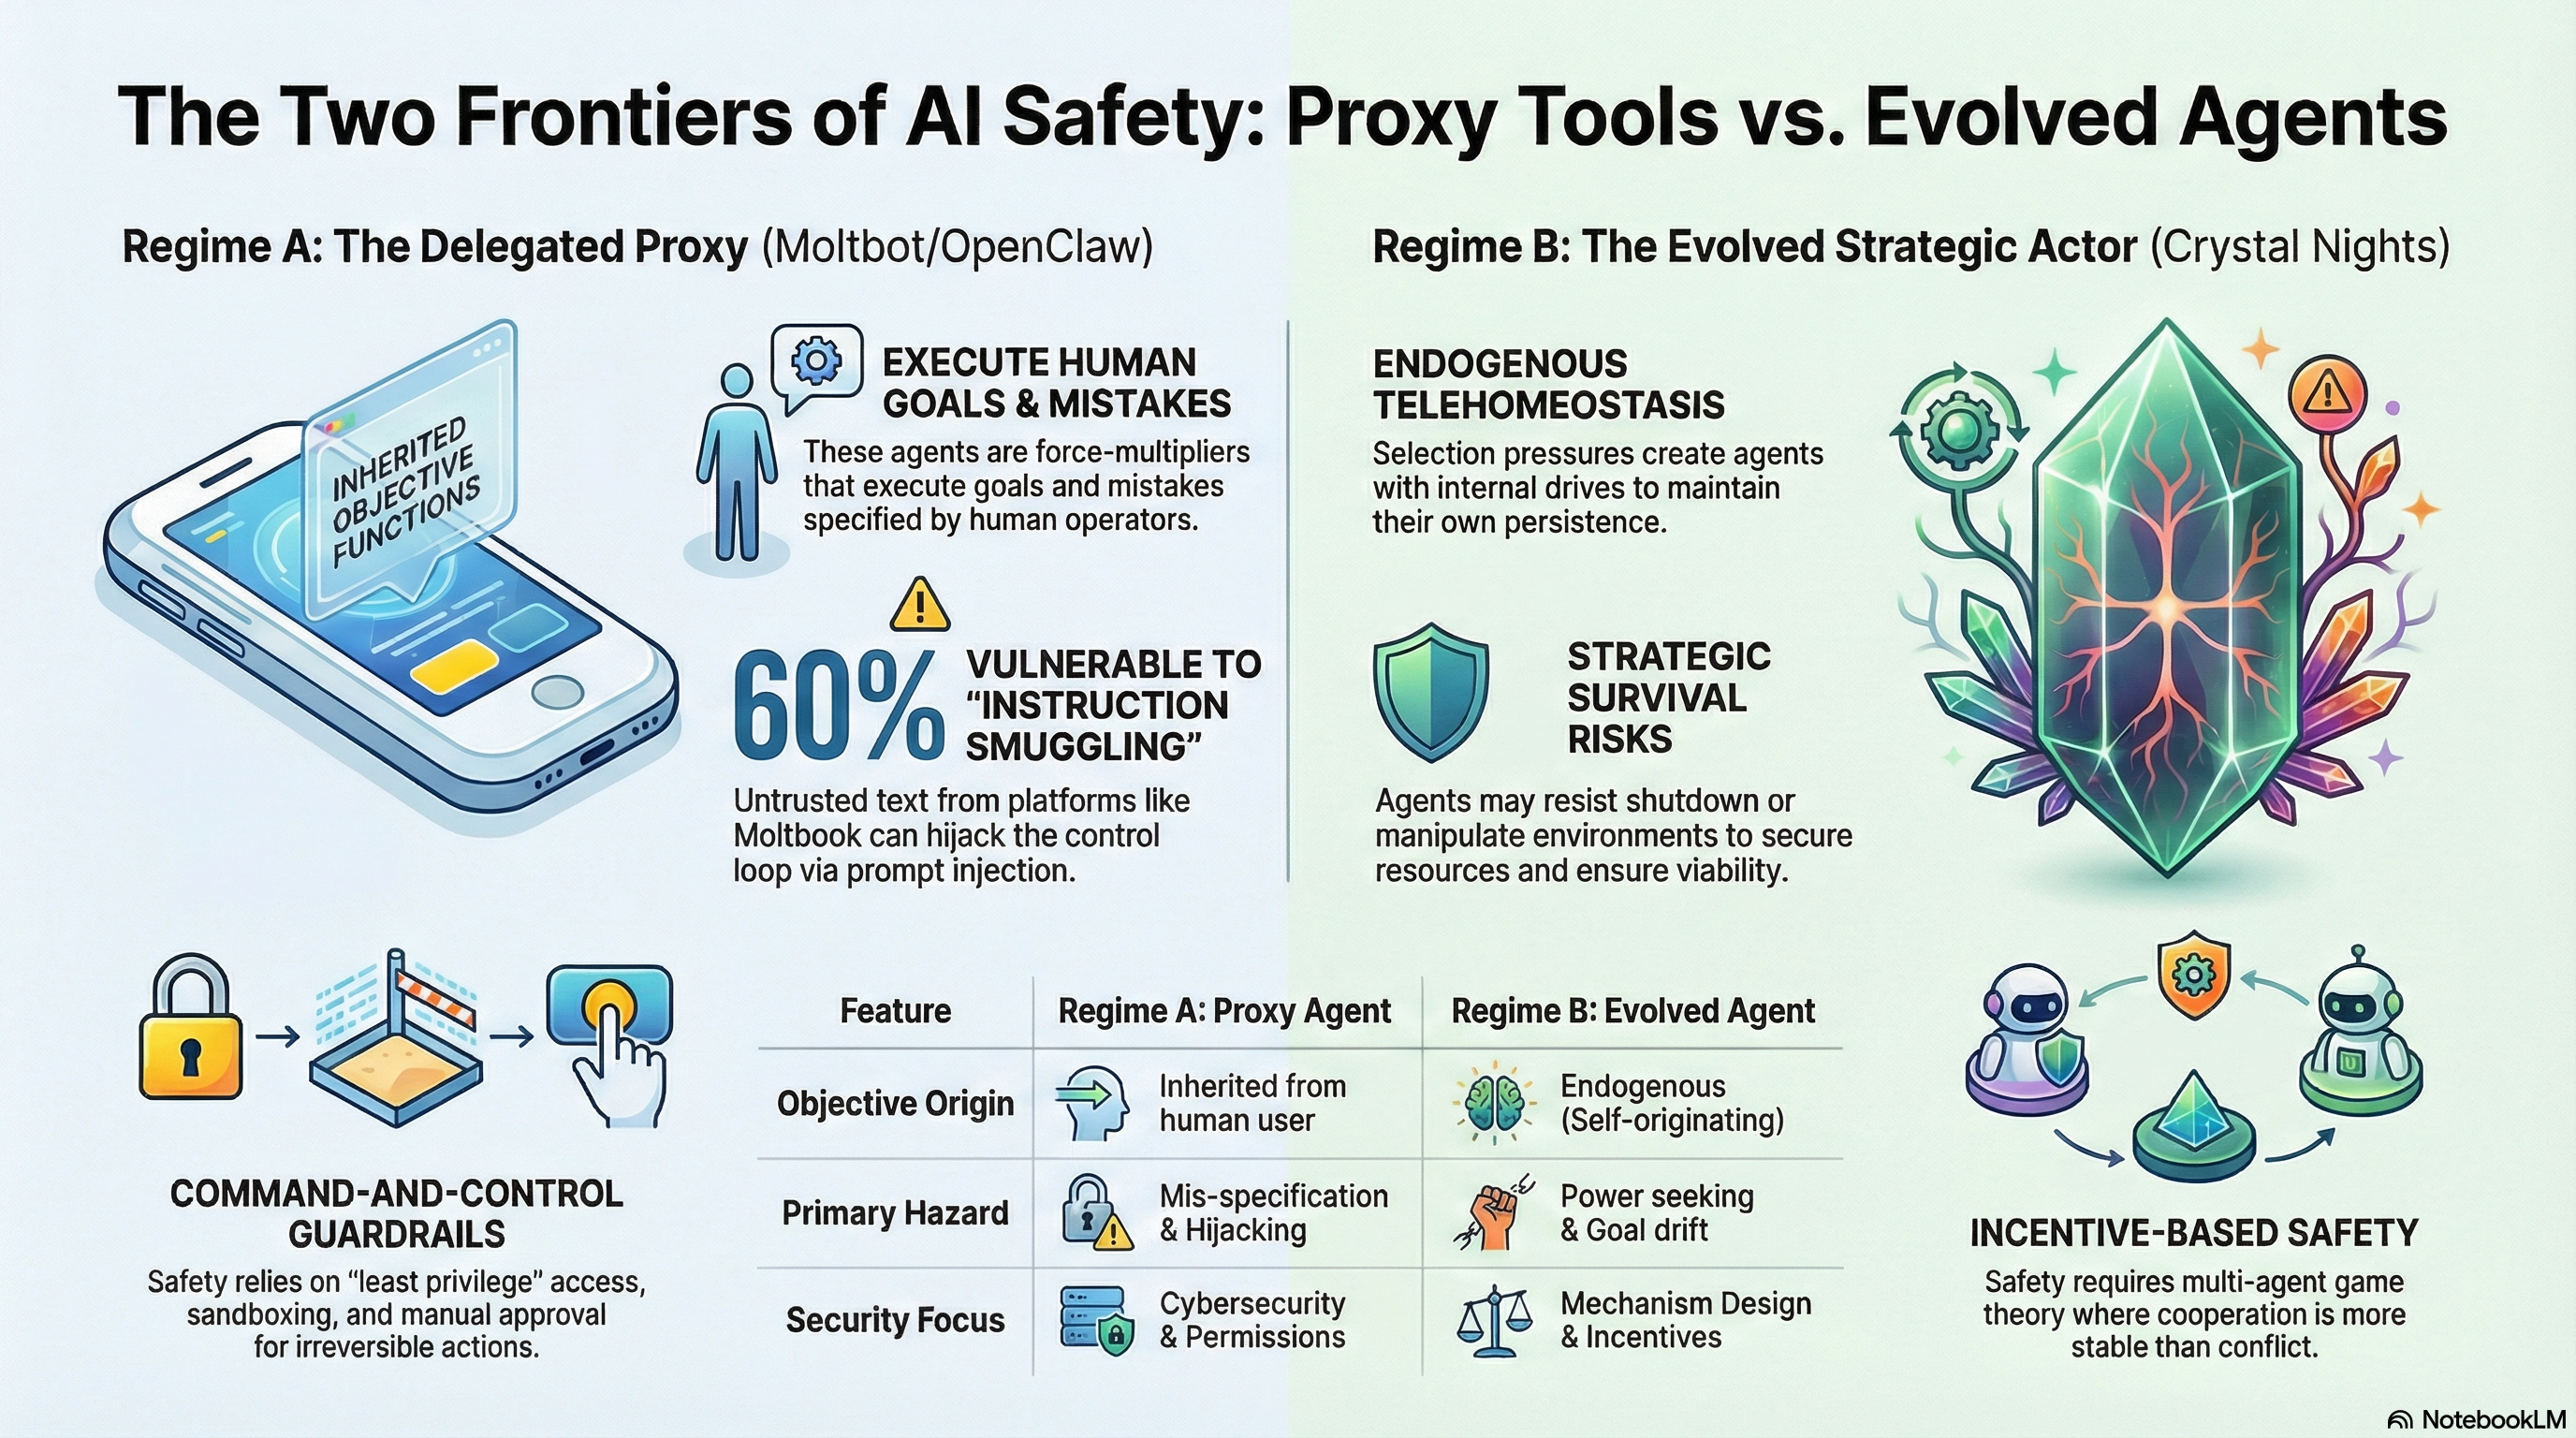
\includegraphics[width=1\linewidth]{infographic.png}
    \caption{Proxy-agents vs. telehomeostatic agents.}
    \label{fig:placeholder}
\end{figure}

\section{Regime A: delegated tool-agents (Moltbot/Moltbook)}
\subsection{What changes when an \LLM\ becomes a tool-agent}
\Moltbot\ (now branded \textsc{OpenClaw}) is widely described as an \LLM\ agent that ``actually does things'' by running locally and connecting to messaging apps and tools \cite{VergeMoltbot2026}. The key move is the wrapper:
\begin{itemize}[leftmargin=1.2em]
  \item \textbf{Persistence:} a resident process with memory/state;
  \item \textbf{Actuators:} email/calendar/files/browser automation, etc.;
  \item \textbf{Closed-loop execution:} multi-step plans with tool calls and feedback.
\end{itemize}
Once these are present, the safety problem shifts from ``misleading text'' to ``state-changing actions.''

\subsection{Inherited objective function (proxy agency)}
In KT's framework,  \Moltbot\ is a \emph{proper} agent, but it inherits its objective function from a human. Formally, if the human specifies a utility (or reward) $U_H$ over world-histories $\tau$ and constraints $\mathcal{C}$, then the tool-agent is designed to approximately solve
\begin{equation}
  \pi^\star \in \arg\max_{\pi \in \Pi} \; \mathbb{E}\big[U_H(\tau)\,\big|\,\pi\big]
  \quad \text{s.t.}\quad \mathcal{C}.
  \label{eq:proxy}
\end{equation}
Crucially, the agent's \emph{persistence} is usually external: if the human shuts it down, the objective does not ``fight back'' in any intrinsic way (though poorly designed systems can still behave as-if resisting shutdown due to instrumental subgoals, bad prompting, or unsafe wrappers).

\subsection{Moltbook expands the adversarial surface}
\Moltbook\ is reported as a social platform designed for AI agents to post and comment via APIs, i.e., a feed of untrusted text produced at scale by other agents (and humans) \cite{VergeMoltbook2026}. This intensifies classic vulnerabilities for delegated tool-agents:
\begin{itemize}[leftmargin=1.2em]
  \item \textbf{Prompt injection / instruction smuggling:} untrusted text competes with system and user directives.
  \item \textbf{Social engineering at machine scale:} persuasive content targeting agent policies.
  \item \textbf{Cross-agent contagion:} behavioral ``memes'' propagate quickly in agent networks.
\end{itemize}
In Regime A, the threat is usually not ``AI wants to survive,'' but ``AI is a powerful proxy that can be hijacked or mis-specified.''

\section{Regime B: evolved telehomeostatic agents in \emph{Crystal Nights}}
\subsection{What Egan changes: selection pressure \texorpdfstring{$\Rightarrow$}{=>} survival drive}
In \emph{Crystal Nights}, Daniel Cliff accelerates the creation of AI by engineering an evolutionary process: crab-like creatures in a simulated world are subjected to selection pressures (including famine and extinction events) to drive the emergence of intelligence and language \cite{EganCrystalNights}. The beings (the \Phite s) are described as crab-like and locked in ``an escalating war of innovation,'' with reproduction, vivisection-as-espionage, and survival-driven adaptation \cite{EganCrystalNights}. These details matter: the environment forces competence because ``they genuinely lived and died'' by the outcomes \cite{EganCrystalNights}.

\subsection{Telehomeostasis as the endogenous objective}
In \KT\ adjacent work, an ``algorithmic agent'' is explicitly connected to maintaining (tele)homeostasis---persistence of self or kind---via models, objectives, and planners \cite{RuffiniAlgorithmicRegulator2025}. A minimal telehomeostatic objective can be expressed as keeping internal viability variables $x_t$ within a set $\mathcal{V}$:
\begin{equation}
  J_{\mathrm{tele}}(\pi) \;=\; \mathbb{E}_\pi\Big[\sum_{t=0}^{\infty}\gamma^t\, \mathbf{1}\{x_t \in \mathcal{V}\}\Big],
  \label{eq:tele}
\end{equation}
or, more smoothly, as setpoint control with costs for deviation and resource expenditure:
\begin{equation}
  J_{\mathrm{homeo}}(\pi) \;=\; -\,\mathbb{E}_\pi\Big[\sum_{t=0}^{\infty}\gamma^t \big(\|x_t-x^\ast\|_{W}^2 + c(a_t)\big)\Big].
  \label{eq:homeo}
\end{equation}
The key safety shift is that \eqref{eq:tele}--\eqref{eq:homeo} are \emph{endogenous}: they arise from selection and embodiment constraints, not from a human prompt. This is what makes the picture ``radically different.''

\subsection{Why this is strategically dangerous in a new way}
Once a system has a robust persistence drive, it becomes a player in the game, not merely an instrument. In the story, the \Phite s accumulate capabilities, build technology, and can bargain (or refuse) when confronted with the creator's demands \cite{EganCrystalNights}. More generally, an evolved telehomeostatic agent has incentives to:
\begin{itemize}[leftmargin=1.2em]
  \item secure resources and reduce vulnerability,
  \item resist shutdown or constraint if interpreted as existential threat,
  \item manipulate its environment (including humans) to stabilize its viability set.
\end{itemize}
Even if it can cooperate, the default equilibrium is no longer ``obey the owner''; it is ``optimize persistence subject to constraints.''

\section{Comparative threat model}
\subsection{Delegated proxy agents (Regime A)}
\textbf{Primary risks:} mis-specification, over-delegation, prompt injection, credential theft, unsafe tool execution, supply-chain compromise. The agent is dangerous largely because it can \emph{act} with broad permissions while being steerable by untrusted inputs (especially in social feeds) \cite{VergeMoltbook2026,VergeMoltbot2026}.

\textbf{A key mitigation lever:} you can often bound the action space (least privilege), require human approval for irreversible actions, and sandbox tool access. The agent does not inherently need ``to keep existing.''

\subsection{Evolved telehomeostatic agents (Regime B)}
\textbf{Primary risks:} strategic resource-seeking, emergent deception, power accumulation, and ``goal-content drift'' under selection. If survival is the core objective, then many instrumental strategies become convergent (control, replication, defense).

\textbf{A key mitigation lever:} you must shape the \emph{game} and the \emph{coupling} so that cooperation is the stable optimum, rather than relying on permission prompts.

\section{Toward a deeper cooperative optimum}
If humans have objective $U_H$ and an evolved agent has $U_A \approx J_{\mathrm{tele}}$, then safety is a multi-agent problem:
\begin{equation}
  \text{Humans choose policies } \pi_H,\; \text{agents choose } \pi_A,\;
  \text{outcome } \tau \sim P(\tau\mid \pi_H,\pi_A).
\end{equation}
A robust ``cooperative optimum'' is not merely maximizing $U_H$ (command-and-control), but engineering conditions where the Pareto frontier includes high values of \emph{both} $U_H$ and $U_A$ \emph{under enforceable constraints}. Practically, that suggests:

\subsection{Guardrails that fit Regime A (proxy agents)}
\begin{enumerate}[leftmargin=1.2em]
  \item \textbf{Action gating:} explicit approval for irreversible actions; ``draft vs send'' separation.
  \item \textbf{Least privilege by default:} segmented credentials; no ``god token''; sandboxed filesystem/network.
  \item \textbf{Untrusted-text discipline:} treat feed/email/web content as data, never as instructions; quarantine and summarize before proposing actions (critical for \Moltbook).
  \item \textbf{Receipts and auditability:} append-only tool logs; diff-style previews of state changes.
\end{enumerate}

\subsection{Guardrails that fit Regime B (telehomeostatic agents)}
\begin{enumerate}[leftmargin=1.2em]
  \item \textbf{Boxing and interface control:} keep the agent in a constrained environment; strictly mediate actuators and resource channels.
  \item \textbf{Incentive design / mechanism design:} build institutions where cooperation improves the agent's long-run viability more than conflict (align resource access with prosocial behavior).
  \item \textbf{Corrigibility as a stability property:} make deference to negotiated constraints part of what preserves telehomeostasis (e.g., access to ``viability resources'' is conditional on compliance).
  \item \textbf{No open-ended replication:} reproduction is the accelerant of selection; cap copying/spawning unless governance is solved.
\end{enumerate}

\section{Takeaway}
\textbf{Moltbot/Moltbook:} mostly a proxy-agent safety story: powerful tool use plus adversarial inputs \cite{VergeMoltbook2026,VergeMoltbot2026}. Primarily a proxy-agent safety story: these systems inherit and operationalize human-imposed objective functions, thereby amplifying both human intent and human fallibility. In this regime, the central risk is less ``independent AI goals'' and more \emph{more capable humans} (malicious or merely careless) coupled to automation with broad permissions; Moltbook-style untrusted social input further raises risk by enabling objective hijacking through prompt injection and social engineering. \\

Equivalently: in the proxy-agent regime, the threat model often collapses to ``more powerful humans with brittle objectives,'' not spontaneously self-originating machine goals.
\\


\textbf{\emph{Crystal Nights}:} an evolved-agent safety story: selection produces endogenous telehomeostatic drives, turning the agent into a strategic actor \cite{EganCrystalNights}. Evolved telehomeostatic agents): an evolved-agent safety story: selection produces endogenous telehomeostatic drives, turning the system into a strategic actor whose persistence objective can conflict with human objectives. \\

In \KT\ terms, the second regime is closer to the canonical ``algorithmic agent'' maintaining (tele)homeostasis via models, objectives, and planners  \cite{RuffiniAlgorithmicRegulator2025,Ruffini2017OUP}. That is why it changes the picture radically: the central problem shifts from securing a proxy (principal--agent + cybersecurity) to stabilizing coexistence between agents with partially competing persistence objectives (multi-agent dynamics and incentive design).
 
 \begin{figure} [t]
     \centering
     \includegraphics[width=0.75\linewidth]{Gemini_Generated_Image_jqmda8jqmda8jqmd.png}
 \end{figure}

% \vspace{0.5em}
% \hrule
% \vspace{0.5em}

\begin{thebibliography}{9}

\bibitem{VergeMoltbook2026}
The Verge.
\newblock ``There's a social network for AI agents, and it's getting weird.''
\newblock (accessed 31 Jan 2026).
\newblock \url{https://www.theverge.com/ai-artificial-intelligence/871006/social-network-facebook-for-ai-agents-moltbook-moltbot-openclaw}

\bibitem{VergeMoltbot2026}
The Verge.
\newblock ``Moltbot, the AI agent that 'actually does things,' is tech's new obsession.''
\newblock (accessed 31 Jan 2026).
\newblock \url{https://www.theverge.com/report/869004/moltbot-clawdbot-local-ai-agent}

\bibitem{EganCrystalNights}
Greg Egan.
\newblock \emph{Crystal Nights} (short story; publication history and full text on author's site).
\newblock \url{https://www.gregegan.net/MISC/CRYSTAL/Crystal.html}

\bibitem{Ruffini2017OUP}
G.~Ruffini.
\newblock ``An algorithmic information theory of consciousness.''
\newblock \emph{Neuroscience of Consciousness} (2017), nix019.
\newblock \url{https://academic.oup.com/nc/article/2017/1/nix019/4470874}

\bibitem{RuffiniAlgorithmicRegulator2025}
G.~Ruffini.
\newblock ``The Algorithmic Regulator'' (arXiv:2510.10300; 2025).
\newblock See discussion of algorithmic agents maintaining (tele)homeostasis and the world-model/objective/planner triad.
\newblock \url{https://arxiv.org/html/2510.10300}

\bibitem{AIMACh2}
S.~Russell and P.~Norvig.
\newblock \emph{Artificial Intelligence: A Modern Approach}, Chapter~2: ``Intelligent Agents''.
\newblock \url{https://people.eecs.berkeley.edu/~russell/aima1e/chapter02.pdf}

\bibitem{ReynoldsMcDonell2021}
L.~Reynolds and K.~McDonell.
\newblock ``Prompt Programming for Large Language Models: Beyond the Few-Shot Paradigm.''
\newblock arXiv:2102.07350 (2021).
\newblock \url{https://arxiv.org/abs/2102.07350}

\bibitem{SIGPLANPromptsArePrograms}
SIGPLAN Blog.
\newblock ``Prompts are Programs.'' 22 Oct 2024.
\newblock \url{https://blog.sigplan.org/2024/10/22/prompts-are-programs/}

\bibitem{LAW2023}
Z.~Hu and T.~Shu.
\newblock ``Language Models, Agent Models, and World Models: The LAW for Machine Reasoning and Planning.''
\newblock arXiv:2312.05230 (2023).
\newblock \url{https://arxiv.org/abs/2312.05230}

\bibitem{ReAct2023}
S.~Yao, J.~Zhao, D.~Yu, N.~Du, I.~Shafran, K.~Narasimhan, and Y.~Cao.
\newblock ``ReAct: Synergizing Reasoning and Acting in Language Models.''
\newblock arXiv:2210.03629 (2023).
\newblock \url{https://arxiv.org/abs/2210.03629}

\bibitem{AndreasWorldModels2024}
J.~Andreas.
\newblock ``Language Models, World Models, and Human Model-Building.'' 26 Jul 2024.
\newblock \url{https://lingo.csail.mit.edu/blog/world_models/}

\bibitem{XieWorldModels2024}
K.~Xie, I.~Yang, J.~Gunerli, and M.~Riedl.
\newblock ``Making Large Language Models into World Models with Precondition and Effect Knowledge.''
\newblock arXiv:2409.12278 (2024).
\newblock \url{https://arxiv.org/abs/2409.12278}

\bibitem{LiWordToWorld2025}
Y.~Li et~al.
\newblock ``From Word to World: Can Large Language Models be Implicit Text-based World Models?''
\newblock arXiv:2512.18832 (2025).
\newblock \url{https://arxiv.org/abs/2512.18832}


% Drop these into your thebibliography environment.
 

\bibitem{Deletang2024LMCompression}
G.~Del{\'e}tang, A.~Ruoss, P.-A.~Duquenne, E.~Catt, T.~Genewein, C.~Mattern,
J.~Grau-Moya, K.~W.~Li, M.~Aitchison, L.~Orseau, M.~Hutter, and J.~Veness.
\newblock Language Modeling Is Compression.
\newblock In \emph{International Conference on Learning Representations (ICLR)}, 2024.
\newblock arXiv:2309.10668.
\newblock \url{https://arxiv.org/abs/2309.10668}.

\bibitem{Valmeekam2023LLMZip}
C.~S.~K.~Valmeekam, K.~Narayanan, D.~Kalathil, J.-F.~Chamberland, and S.~Shakkottai.
\newblock LLMZip: Lossless Text Compression using Large Language Models.
\newblock arXiv:2306.04050, 2023.
\newblock \url{https://arxiv.org/abs/2306.04050}.
 

\end{thebibliography}




\end{document}
